\documentclass[12pt]{article}
\usepackage[english]{babel}
\usepackage{natbib}
\usepackage{url}
\usepackage[utf8x]{inputenc}
\usepackage{amsmath}
\usepackage{graphicx}
\graphicspath{{images/}}
\usepackage{parskip}
\usepackage{fancyhdr}
\usepackage{vmargin}
\usepackage{subfig}
\usepackage{tikz}
\usepackage[normalem]{ulem}
\usepackage{amssymb}
\usetikzlibrary{shapes.geometric, arrows}
\tikzstyle{startstop} = [rectangle, rounded corners, minimum width=2cm, minimum height=0.5cm,text centered, draw=black, fill=red!30]
\tikzstyle{io} = [trapezium, trapezium left angle=70, trapezium right angle=110, minimum width=3cm, minimum height=0.5cm, text centered, draw=black, fill=blue!30]
\tikzstyle{process} = [rectangle, minimum width=3cm, minimum height=0.5cm, text centered, draw=black, fill=orange!30]
\tikzstyle{decision} = [diamond, minimum width=2cm, minimum height=0.5cm, text centered, draw=black, fill=green!30]
\tikzstyle{arrow} = [thick,->,>=stealth]
\usetikzlibrary{positioning,fit,calc}
\tikzset{block/.style={draw,thick,text width=2cm,minimum height=1cm,align=center},
         line/.style={-latex}
}

\setmarginsrb{3 cm}{2.5 cm}{3 cm}{2.5 cm}{1 cm}{1.5 cm}{1 cm}{1.5 cm}

\title{Cooperative Localization Using Posterior Linearization Belief Propagation}								% Title
\author{SHIVRAM MEENA\\
		SHASHI KANT GUPTA \\
		MAMILLA SIVASANKAR \\
		PRADEEP KUMAR \\
		ALLAPARTHI VENKATA SATYA VITHIN \\}								% Author
\date{\today}											% Date

\makeatletter
\let\thetitle\@title
\let\theauthor\@author
\let\thedate\@date
\makeatother

\pagestyle{fancy}
\fancyhf{}

\rhead{Group-9}
\cfoot{\thepage}

\begin{document}

%%%%%%%%%%%%%%%%%%%%%%%%%%%%%%%%%%%%%%%%%%%%%%%%%%%%%%%%%%%%%%%%%%%%%%%%%%%%%%%%%%%%%%%%%

\begin{titlepage}
	\centering
    \vspace*{0.5 cm}

	\textsc{\Large Term Paper}\\[0.5 cm]				% Course Code
					% Course Name
	\rule{\linewidth}{0.2 mm} \\[0.4 cm]
	{ \huge  \thetitle}\\
	\rule{\linewidth}{0.2 mm} \\[4 cm]
	\textsc{\large Group-9}\\[0.5 cm]
	\begin{minipage}{0.7\textwidth}
		\begin{flushleft} \large
			\emph{Author:}\\
			\theauthor
			\end{flushleft}
			\end{minipage}~
			\begin{minipage}{0.4\textwidth}
			\begin{flushright} \large
			\emph{Student Number:} \\
			150686 \\
160645 \\
17104091 \\
18104074 \\
18104265\\							% Your Student Number
		\end{flushright}
	\end{minipage}\\[2 cm]
	\textsc{\large Statistical Signal Processing EE602A}\\[0.5 cm]
	{\large \thedate}\\[2 cm]

	\vfill

\end{titlepage}

%%%%%%%%%%%%%%%%%%%%%%%%%%%%%%%%%%%%%%%%%%%%%%%%%%%%%%%%%%%%%%%%%%%%%%%%%%%%%%%%%%%%%%%%%

\tableofcontents
\pagebreak

%%%%%%%%%%%%%%%%%%%%%%%%%%%%%%%%%%%%%%%%%%%%%%%%%%%%%%%%%%%%%%%%%%%%%%%%%%%%%%%%%%%%%%%%%

\section{AIM/OBJECTIVE}
  To infer the positions of the sensor nodes in cooperative fashion using the posterior linearization belief propagation (PLBP) algorithm with nonlinear measurements.
\section{PROBLEM DEFINITION}
In cooperative localization, there are some anchor nodes whose positions are known accurately. The remaining nodes infer their positions based on intercommunication between themselves, each node is connected to some other nodes which pass some messages to it for example distance. The measurements are generally non linear. Hence, we linearize the model by using statistical linearization using Sigma Points. Belief Propagation algorithm will be applied on the linearized posteriors to update the node position using Kalman filter updates. Strategies which increases the computational efficiency and noise robust are required.
\section{SYSTEM MODEL/METHODOLOGY}
A graph $G=(V,E)$ is formed by a collection of vertices/nodes $V=(1,...,m)$, where $m$ is the number of nodes, and a collection of edges $E⊂V×V$. Each edge consists of a pair of nodes $(i,j) ∈ E$. The state of node $i$ is represented by $x_i∈R^{n_x}$\\

We assume $x_{i}$  has Gaussian PDF\\

 \begin{equation}
p_{i}(x_{i}) =\mathcal {N}\left(x_{i};\overline{x}_{i},P_{i}\right)
\end{equation}
With $x_{i}$ representing the state of the node and  $\overline{x}_{i},P_{i}$ are mean and co-variance respectively\\

\begin{enumerate}
\item Defining the system model.
	\begin{equation}
z_{i,j}=h_{i,j}(x_{i},x_{j})+n_{i,j}
\end{equation}
$h_{i,j}$ represent the measurement fuction between two nodes i and j. $n_{i,j}$ is the noise measurement. \\

\item Nonlinear measurement function.
	\begin{equation}
	h_{i,j}(x_{i},x_{j})=\sqrt{(p_{x,i}-p_{x,j})^{2}+(p_{y,i}-p_{y,j})^{2}}
	\end{equation}

\item Linearization model of non linear measurements
\begin{equation}
h_{i,j} \approx A_{i,j}^{1}x_{i}+A_{i,j}^{2}x_{j}+b_{i,j}+e_{i,j}
\end{equation}

\begin{enumerate}
\item Select m sigma points $\chi_{0},\chi_{1},\cdots,\chi_{m}$.
\item Propagate sigma points $Z_{j}=h(\chi_{j})$
\item Compute mean and variance.
\begin{equation}

\overline{z}=\sum _{j=1}^{m}\omega _{j}\mathcal {Z}_{j}
\end{equation}
\begin{equation}
\Psi =\sum _{j=1}^{m}\omega _{j}\left(\mathcal
 {X}_{j}-\overline{x}\right)\left(\mathcal {Z}_{j}-\overline{z}\right)^{T}
\end{equation}
\begin{equation}
\Phi =\sum _{j=1}^{m}\omega _{j}\left(\mathcal {Z}_{j}-\overline{z}\right)\left(\mathcal {Z}_{j}-\overline{z}\right)^{T}
\end{equation}
\begin{equation}
\begin{split}
 A^{\;+\;}=&\Psi ^{T}P^{-1} \\
 b^{\;+\;}=&\overline{z}-A^{\;+\;}\overline{x}\\
 \Omega ^{\;+\;}=&\Phi -A^{\;+\;}P\left(A^{\;+\;}\right)^{T}
 \end{split}
\end{equation}
\end{enumerate}


\item Belief propagation on linearized model.
\begin{enumerate}

 \item  The message $ \mu_{i \rightarrow j}$ from node i to j is given as
  \begin{equation}
\mu_{i \rightarrow j} \propto \int l_{i,j}(z_{i,j}|x_{i},x_{j})\mathcal{N} (x_{ i };\bar{x}_{ i },P_{i})\prod_{p \in n(i)\setminus \{ j \} } \mu_{p\rightarrow i}(x_{i}) dx_{i}
\end{equation}
\item under approximation

\begin{equation}
   \mu_{i \rightarrow j}(x_{j}) \propto \mathcal{N} (\alpha_{i \rightarrow j};H_{i \rightarrow j}x_{j},\tau_{i \rightarrow j})
\end{equation}
 \begin{equation}
   \alpha_{i \rightarrow j}=z_{i,j}-A^{1}_{i,j}\bar{x}_{i \rightarrow j}-b_{i,j}
\end{equation}
 \begin{equation}
 H_{i \rightarrow j}=A^{2}_{i,j}
\end{equation}
 \begin{equation}
 \tau_{i \rightarrow j}=R_{i,j}+\Omega_{i,j}+A^{1}_{i,j}P_{i \rightarrow j}(A^{1}_{i,j})^{T}
\end{equation}

\end{enumerate}

\end{enumerate}
\pagebreak
\subsection{Algorithm flow}
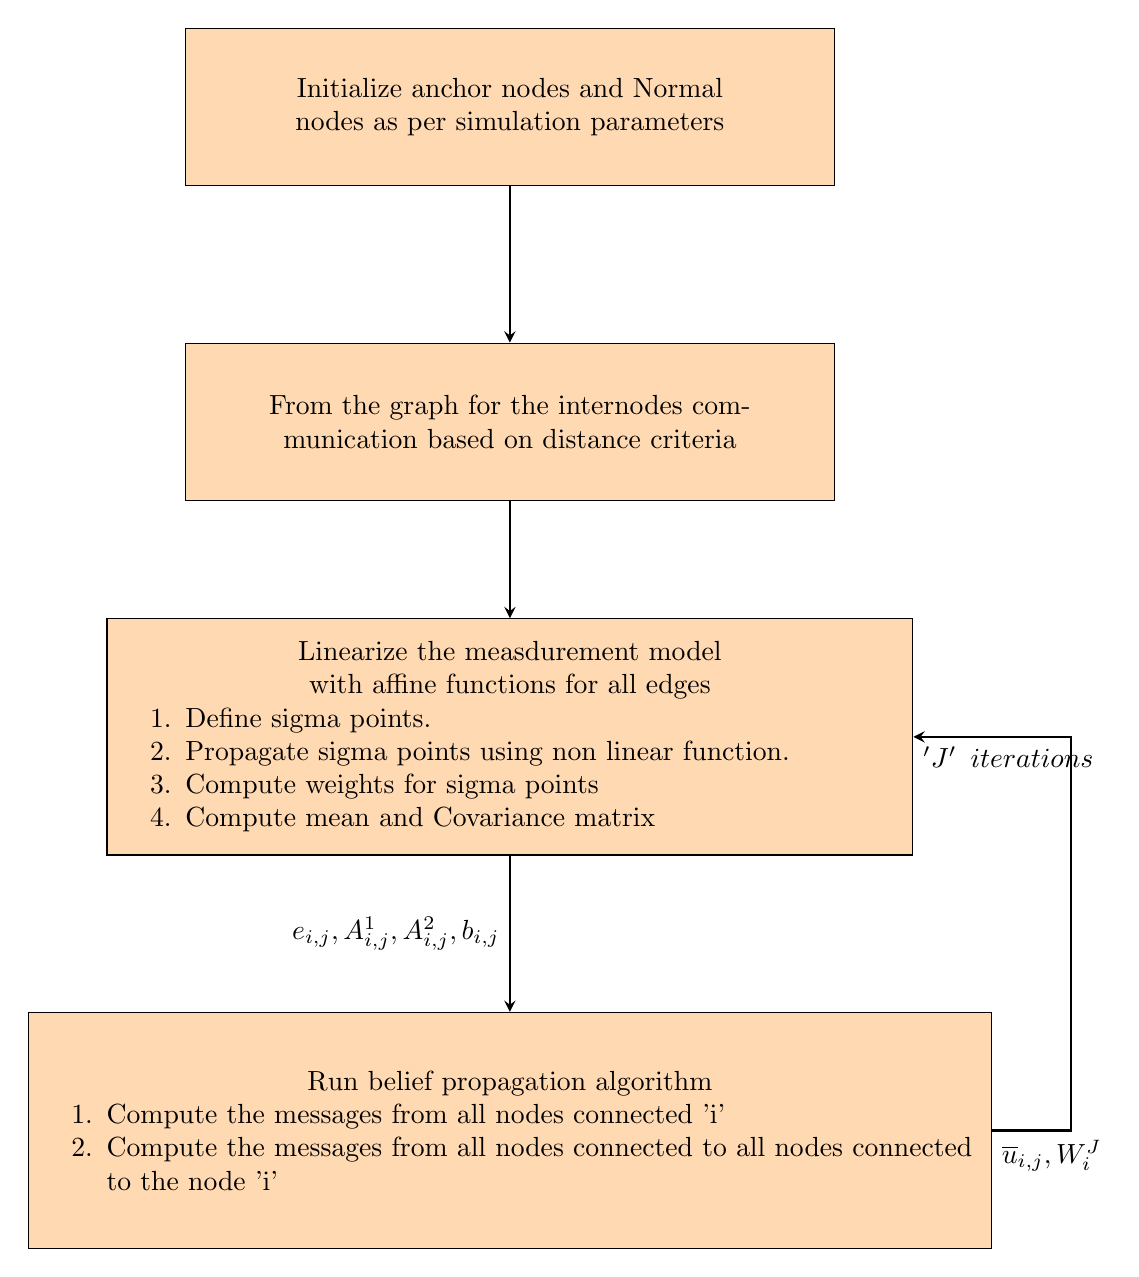
\begin{tikzpicture}[node distance=2cm]
\centering
\node (pro1) [process,rectangle, minimum height=2cm, text centered, text width=8cm, draw=black, fill=orange!30] {Initialize anchor nodes and Normal nodes as per simulation parameters };
\node (pro4) [process,below of=pro1, yshift=-2cm,rectangle, minimum height=2cm, text centered, text width=8cm, draw=black, fill=orange!30] {From the graph for the internodes
communication based on distance criteria };
\node (pro5) [process,below of=pro4, yshift=-2cm,rectangle, minimum height=3cm, text centered, text width=10cm, draw=black, fill=orange!30] {Linearize the measdurement model with affine functions for all edges
\begin{enumerate}
\item Define sigma points.
\item Propagate sigma points using non linear function.
\item Compute weights for sigma points
\item Compute mean and Covariance matrix
\end{enumerate}};
\node (pro6) [process,below of=pro5, yshift=-3cm,rectangle, minimum height=3cm, text centered, text width=12cm, draw=black, fill=orange!30] {Run belief propagation algorithm
\begin{enumerate}
\item Compute the messages from all nodes connected 'i'
\item Compute the messages from all nodes connected to all nodes connected to the node 'i'

\end{enumerate} };

\draw [arrow] (pro1) -- (pro4);
\draw [arrow] (pro4) -- (pro5);
\draw [arrow] (pro5) -- node[anchor=east] {$e_{i,j},A^{1}_{i,j},A^{2}_{i,j},b_{i,j}$}(pro6);
\draw  [arrow,->] (pro6.east)--++(+1.0cm,0)|-node[anchor=west,below right]{}(pro5);
\draw (pro6.east)node[anchor=west,below right]{$\overline{u}_{i,j},W_{i}^{J}$};
\draw (pro5.east)node[anchor=west,below right]{$ 'J' \,\,\, iterations $};
\end{tikzpicture}


%\begin{figure}[h]
%\centering
%\subfloat[]{\includegraphics[width=1\textwidth]{alg_flow.png}}\\
%
%\caption{ algorithm flow }
%\label{carrdh}
%\end{figure}
\newpage

\section{MATLAB SIMULATIONS AND RESULTS}


A MATLAB simulation is performed according to the system model described below.\\
\begin{align*}
  Area		&	:&  100 m X 100 m\\
Number\;of\; Anchor\; nodes	&	:&   13\\
Number\; of\; Normal \;nodes      	&	:&   100\\
Variance\; of\; Normal\; Nodes	&	:&  100 m\\
Variance\; of\; Anchor\; Nodes	&	:& 0.01 m\\
Number \;of\; Iterations 		&	:&  20\\
Range\; Measurement\; error           &	:&  1 m
\end{align*}

\\
Results for the simulation is shown below. Please find the attached Matlab Code in Appendix at the end of this document.

\begin{figure}
  \centering
{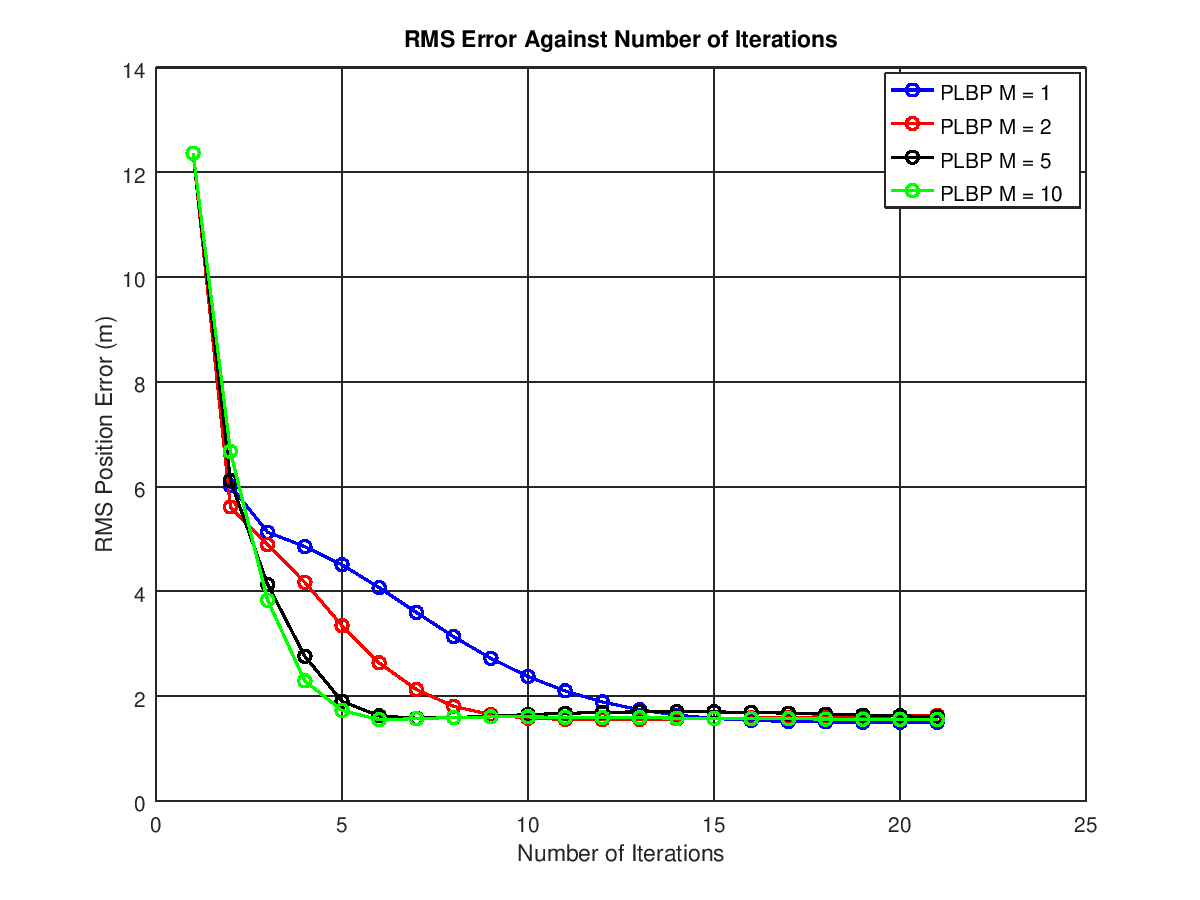
\includegraphics[width=0.8\textwidth]{images/RMSE.png}}
\caption{ RMS error against number of iterations. Performance improves with
M , number of BP iterations per linearisation. }
{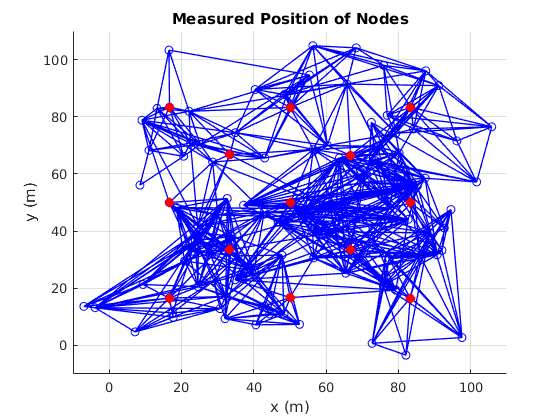
\includegraphics[width=0.8\textwidth]{images/measured.png}}
\caption{ Position of measured nodes i.e. with noise. Red circles indicate the positions of 13
anchor nodes, blue circles the positions of the other 100 nodes and blue lines
the edges of the graph. Communication radius is 20 m.}

\end{figure}

\begin{figure}
  \centering
{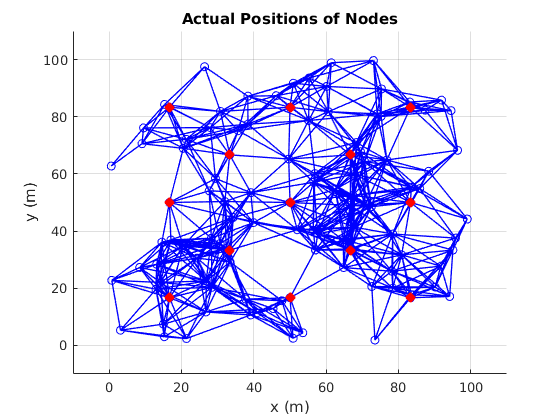
\includegraphics[width=0.8\textwidth]{images/actual.png}}
{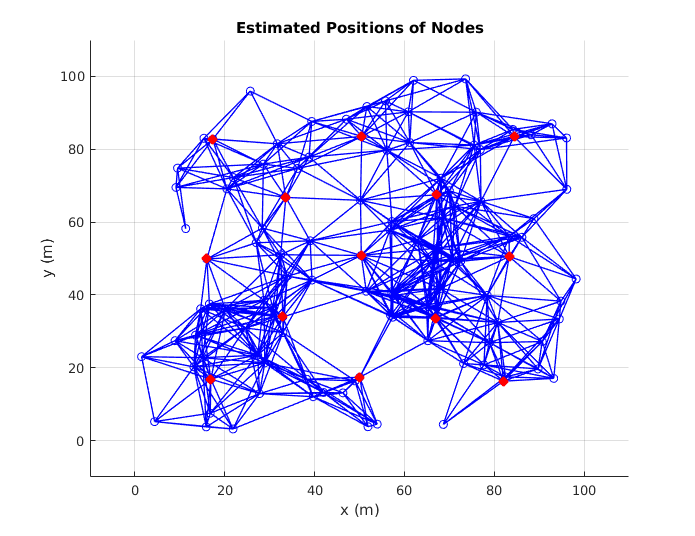
\includegraphics[width=0.8\textwidth]{images/est.png}}
\caption{ Comparison of actual node position and estimated node position using PLBP algorithm. }
\end{figure}

\newpage






\section{CONCLUSION}
 Posterior Linearizaation Belief propagation algorithm is used to infer the positions of the unknown nodes in a cooperative manner in a wireless sensor network with less computational complexity.


\newpage
\section{References}
	\begin{itemize}
		\item[1] H. Wymeersch, J. Lien, and M. Win, “Cooperative localization in wireless
networks,” Proc. IEEE, vol. 97, no. 2, pp. 427–450, Feb. 2009.
		\item[2] S. Kianoush, A. Vizziello, and P. Gamba, “Energy-efficient and mobile-
aided cooperative localization in cognitive radio networks,” IEEE Trans.
Veh. Technol., vol. 65, no. 5, pp. 3450–3461, May 2016.
		\item[3] T. V. Nguyen, Y. Jeong, H. Shin, and M. Z. Win, “Least square cooperative
localization,” IEEE Trans. Veh. Technol., vol. 64, no. 4, pp. 1318–1330,
Apr. 2015.
		\item[4] W. Yuan, N. Wu, B. Etzlinger, H. Wang, and J. Kuang, “Cooperative
joint localization and clock synchronization based on Gaussian message
passing in asynchronous wireless networks,” IEEE Trans. Veh. Technol.,
vol. 65, no. 9, pp. 7258–7273, Sep. 2016.
		\item[5] S. J. Julier and J. K. Uhlmann, “Unscented filtering and non-
linear estimation,” in Proc. IEEE, vol. 92, no. 3, pp. 401–422,
Mar. 2004.
		\item[6] F. Meyer, O. Hlinka, and F. Hlawatsch, “Sigma point belief prop-
agation,” IEEE Signal Process. Lett., vol. 21, no. 2, pp. 145–149,
Feb. 2014.
		\item[7] W. Sun and K.-C. Chang, “Unscented message passing for arbitrary con-
tinuous variables in Bayesian networks,” in Proc. 22nd Nat. Conf. Artif.
Intell., 2007, pp. 1902–1903.
		\item[8] S. Särkkä, Bayesian Filtering and Smoothing. Cambridge, MA, USA:
Cambridge Univ. Press, 2013.

		\item[9] D. Bickson, “Gaussian belief propagation: Theory and application,”
Ph.D. dissertation, The Hebrew Univ. Jerusalem, Jerusalem, Israel,
2008.
		\item[10] Q. Su and Y.-C. Wu, “On convergence conditions of Gaussian belief
propagation,” IEEE Trans. Signal Process., vol. 63, no. 5, pp. 1144–1155,
Mar. 2015.			\item[11] P. Tichavsky, C. H. Muravchik, and A. Nehorai, “Posterior Cramér–Rao
bounds for discrete-time nonlinear filtering,” IEEE Trans. Signal Process.,
vol. 46, no. 5, pp. 1386–1396, May 1998.
		\item[12] S. Li, M. Hedley, and I. B. Collings, “New efficient indoor cooperative
localization algorithm with empirical ranging error model,” IEEE J. Sel.
Areas Commun., vol. 33, no. 7, pp. 1407–1417, Jul. 2015.

	\end{itemize}


\newpage

\begin{titlepage}
	\centering
    \vspace*{8 cm}
					% Course Name
	\rule{\linewidth}{0.2 mm} \\[0.4 cm]
	{ \huge  Appendix}\\
	\rule{\linewidth}{0.2 mm} \\[8 cm]


	\vfill

\end{titlepage}













\end{document}
